\documentclass[12pt]{article}
\usepackage[spanish]{babel}
\usepackage[utf8]{inputenc}
%\usepackage{graphicx}
\usepackage[pdftex]{graphicx}

\catcode`\@=11
\def\t@cstrut{{height4.0in depth0.0in width0.0in}}
\def\boundingbox#1{
\box{height4.0in depth0.0in width4.0in #1}
}

\def\AVISO{
\message{USING .jpg files DO NOT FORGET about compiling directly to .pdf 
(pdflatex) and use: graphicx package with pdftex option 
(usepackage[pdftex]{graphicx}).
}}
\catcode`\@=12

\title{Multitasking sobre un AVR}
\author{Traducción de Lamberto Maza Casas}
\date{\today}
\begin{document}

\maketitle

\section{El Tick del RTOS}
Cuando una tarea se suspende a sí misma especif\/ica un periodo de retardo  
(o de ``sleep''). Cada vez que la cuenta de tick es incrementada el 
kernel del RTOS debe revisar para ver si el nuevo valor de la cuenta de 
tick causó que un periodo ha expirado. Cualquier tarea encontrada por el 
kernel del RTOS que tenga un periodo de retardo expirado es puesta en 
estado de lista para correr. Se requerirá un cambio de contexto con el 
tick del RTOS si una tarea puesta en estado lista para correr por la 
rutina de servicio de interrupción de tick (ISR) tiene prioridad más 
alta que la tarea interrumpida por la ISR de tick. Cuando esto ocurre 
el tick del RTOS interrumpirá una tarea, pero retornará a otra. Esto se 
delinea en la siguiente figura:
$$
%\includegraphics[bb=0 0 100 100][scale=0.525]{img/monanAVR_FigPag03.jpg}
%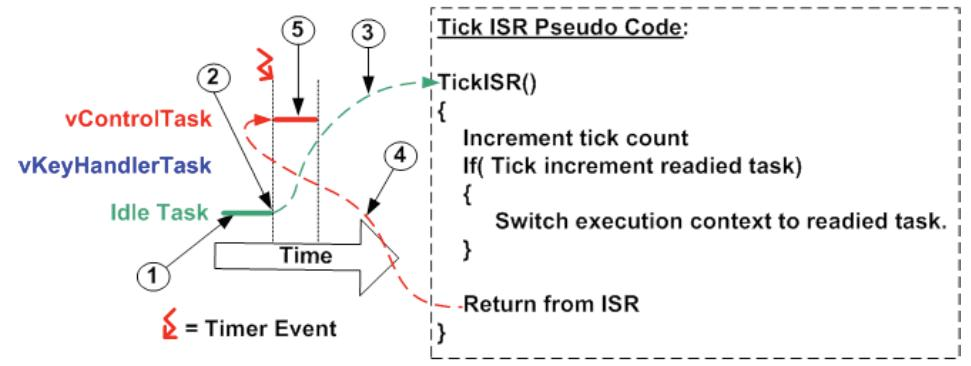
\includegraphics[bb=0 0 50 35]{img/monanAVR_FigPag03.jpg}
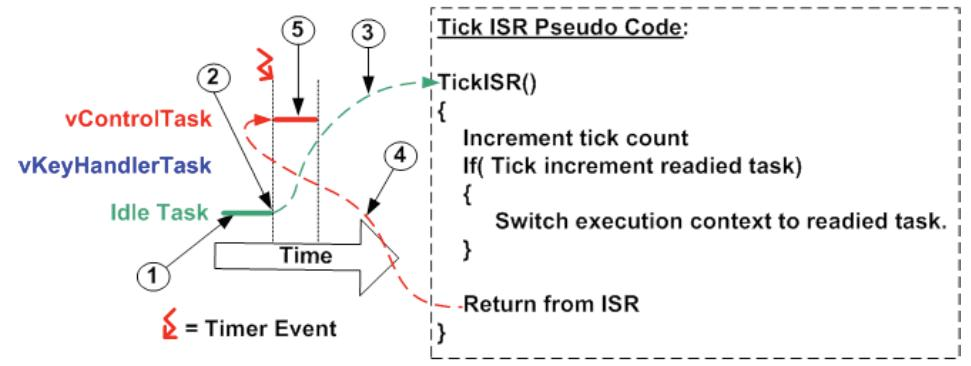
\includegraphics[width=5.5in, height=2.0in]{img/monanAVR_FigPag03.jpg}
%%Using .jpg files do not forget about compiling directly to .pdf 
%%(pdflatex) and use: graphicx package with pdftex option 
%%(\usepackage[pdftex]{graphicx}).
$$
%\end{figure}
En este tipo de diagrama el tiempo se mueve de izquierda a derecha. Las 
líneas coloreadas muestran cuál tarea se está ejecutando en algún 
instante de tiempo particular. Refiriéndose a los números del diagrama 
de arriba:
\begin{itemize}
\item[$\bullet$] En (1) se está ejecutando la tarea idle.
\item[$\bullet$] En (2) ocurre el tick del RTOS, y el control se transfiere 
a la ISR de tick (3).
\item[$\bullet$] La ISR de tick hace que vControlTask se ponga en estado 
lista para correr, y como vControlTask tiene una prioridad más alta que 
la tarea idle, hace el cambio de contexto para la vControlTask.
\item[$\bullet$] Como el contexto de ejecución es ahora el de la 
vControlTask, la salida de la ISR (4) regresa el control a la vControlTask, 
la cual empieza a ejecutarse (5).
\end{itemize}
\section{Generando la interrupción de Tick}
Para generar el tick de RTOS se usa una interrupción compare match del 
periférico timer1 del AVR.

El timer1 se configura para incrementarse a una frecuencia conocida la 
cual es la frecuencia de la entrada de reloj dividida por un prescaler. 
El prescaler es requerido para asegurar que la cuenta del timer no 
presente sobreflujo demasiado rápido. El valor de compare match es 
calculado como el número hasta el cual el timer1 se habrá incrementado 
desde 0 en el periodo tick requerido. Cuando el valor del timer1 
alcanza el valor de compare match la interrupción de compare match se 
ejecutará y el AVR automaticamente reseteará el timer1 a 0 ---de tal 
manera que la siguiente interrupción de tick ocurrirá después de 
exactamente el mismo intervalo. El siguiente es un fragmento del archivo 
{\tt Source/portable/GCC/ATMega323/port.c}
\begin{verbatim}
/* Hardware constants for timer 1. */
#define portCLEAR_COUNTER_ON_MATCH           ( ( uint8_t ) 0x08 )
#define portPRESCALE_64                      ( ( uint8_t ) 0x03 )
#define portCLOCK_PRESCALER                  ( ( uint32_t ) 64 )
#define portCOMPARE_MATCH_A_INTERRUPT_ENABLE ( ( uint8_t ) 0x10 )
\end{verbatim}
La función {\tt prvSetupTimerInterrupt()} también esta def\/inida en \\
{\tt Source/portable/GCC/ATMega323/port.c}
\eject
\begin{verbatim}
/*
 * Setup timer 1 compare match A to generate a tick interrupt.
 */
static void prvSetupTimerInterrupt( void )
{
    uint32_t ulCompareMatch;
    uint8_t ucHighByte, ucLowByte;
    
    /* Using 16bit timer 1 to generate the tick.  Correct fuses must be
    selected for the configCPU_CLOCK_HZ clock. */
    
    ulCompareMatch = configCPU_CLOCK_HZ / configTICK_RATE_HZ;
    
    /* We only have 16 bits so have to scale to get our required tick rate. */
    ulCompareMatch /= portCLOCK_PRESCALER;
    
    /* Adjust for correct value. */
    ulCompareMatch -= ( uint32_t ) 1;
    
    /* Setup compare match value for compare match A.  Interrupts are disabled 
    before this is called so we need not worry here. */
    ucLowByte = ( uint8_t ) ( ulCompareMatch & ( uint32_t ) 0xff );
    ulCompareMatch >>= 8;
    ucHighByte = ( uint8_t ) ( ulCompareMatch & ( uint32_t ) 0xff );
    OCR1AH = ucHighByte;
    OCR1AL = ucLowByte;
    
    /* Setup clock source and compare match behaviour. */
    ucLowByte = portCLEAR_COUNTER_ON_MATCH | portPRESCALE_64;
    TCCR1B = ucLowByte;
    
    /* Enable the interrupt - this is okay as interrupt are currently globally
    disabled. */
    ucLowByte = TIMSK;
    ucLowByte |= portCOMPARE_MATCH_A_INTERRUPT_ENABLE;
    TIMSK = ucLowByte;
}
/*-----------------------------------------------------------*/
\end{verbatim}
\section{{\LARGE $^{\prime}$}Contexto de ejecución{\LARGE $^{\prime}$} 
--una Def\/inición}
Cuando una tarea se ejecuta utiliza los registros del microcontrolador y accede a 
RAM y a ROM justo como cualquier otro programa. Estos recursos juntos (los 
registros, la pila, etc.) comprenden el contexto de ejecución de la tarea.

Una tarea es una pieza de código secuencial que no sabe cuando va a ser suspendida 
(stopped from executing) o continuada (given more processing time) por el RTOS y 
tampoco sabe cuándo esto ha sucedido. Considere el ejemplo de una tarea siendo 
suspendida justamente antes de ejecutar una instrucción que suma los valores 
contenidos en dos registros.
$$
%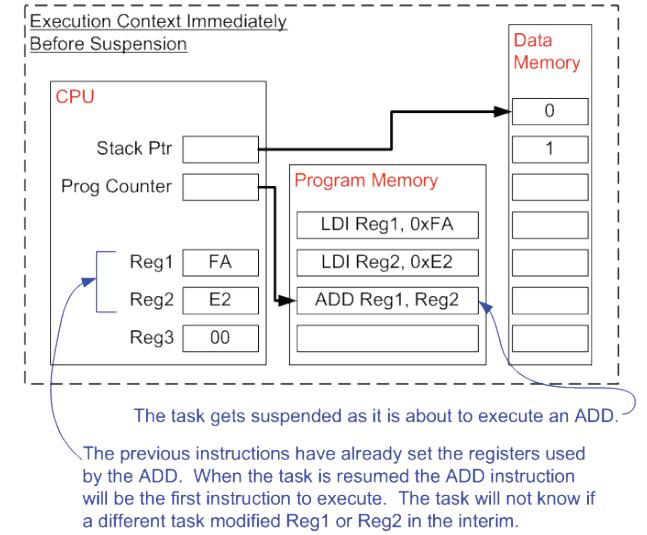
\includegraphics[scale=0.8]{img/monanAVR_FigPag05.jpg}
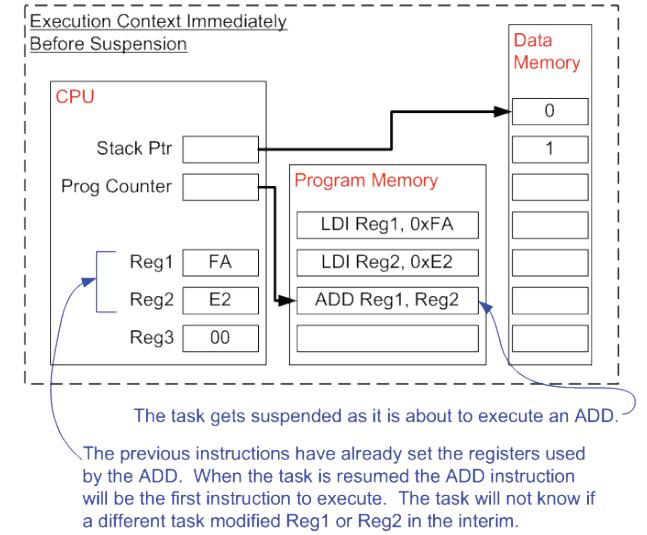
\includegraphics[width=5.5in, height=4.0in]{img/monanAVR_FigPag05.jpg}
$$
Mientras la tarea está suspendida otras tareas se ejecutarán y podrían 
modificar los valores de los registros. Cuando la tarea suspendida 
vuelve a ejecutarse no sabrá que los registros han sido alterados --si 
utilizara los valores modificados la suma resultaría en un valor 
incorrecto.

Para prevenir este tipo de error es esencial que cuando una tarea supendida 
vuelve a ejecutarse tenga un contexto idéntico al que tenía inmediatamente 
antes de su suspención. El kernel de RTOS es responsable de asegurar que 
este sea el caso --y lo hace guardando el contexto de una  tarea cuando 
esta es suspendida. Cuando la tarea es continuada (resumed) su contexto 
guardado  es restaurado por el kernel de RTOS antes de que la tarea 
continue su ejecución. El proceso de guardar el contexto de una tarea 
que va a ser suspendida y restaurar el contexto cuando la tarea va a ser 
continuada es llamado cambio de contexto.
\section{El contexto AVR}
En el microcontrolador AVR el contexto consiste de:
$$
%\includegraphics[scale=1.0]{Iimg/monanAVR_FigPag06.jpg}
\includegraphics[width=5.5in, height=4.0in]{img/monanAVR_FigPag06.jpg}
$$
\begin{itemize}
\item[$\bullet$] Los 32 registros de propósito general. El compilador gcc 
asume que el registro R1 está puesto a cero.
\item[$\bullet$] El registor de estado. El valor del registro de estado 
afecta la ejecución de instrucción y debe ser preservado entre cambios 
de contexto.
\item[$\bullet$] El contador de programa. Cuando una tarea reanuda su 
ejecución debe continuar desde la instrucción que estaba a punto de 
ejecutar justamente antes de su suspensión.
\item[$\bullet$] Los dos registros apuntadores de pila (SPH y SPL).
\end{itemize}

\section{Escribiendo la ISR -- El atributo {\LARGE $^{\prime}$}signal
{\LARGE $^{\prime}$} de GCC}
FreeRTOS gebera la insterrupción de tick de un evento compare match 
sobre el periférico timer1 del AVR. USando GCC la función ISR de tick 
puede ser escrita en C usando la siguiente sintaxis.
\begin{verbatim}
/*
 * Tick ISR for the cooperative scheduler.  All this does is increment the
 * tick count.  We don't need to switch context, this can only be done by
 * manual calls to taskYIELD();
 */
void SIG_OUTPUT_COMPARE1A( void ) __attribute__ ( ( signal ) );
void SIG_OUTPUT_COMPARE1A( void )
{
    xTaskIncrementTick();
}
\end{verbatim}
\section{Código para compare match ISR}
La directiva {\tt $\_\_$attribute$\_\_$ ( ( signal ) )} informa al 
compilador que la función es una ISR y resulta en dos cambios 
importantes para el código de salida del compilador:
\begin{enumerate}
\item El atributo 'signal' asegura que cada registro del AVR que se 
modifica durante la ISR es restaurado a su valor original cuando la ISR 
termina. Esto se requiere dado que el compilador no puede hacer 
suposiciones de cuándo se ejecutara la interrupción. Y por lo tanto no 
se puede optimizar cuáles registros requieren guardarse y cuáles no.
\item El atributo 'signal' también obliga a que se use una instrucción 
'return from interrupt' (RETI) en lugar de la instrucción 'return' (RET). 
El AVR deshabnilita las interrupciones cuando entra a una ISR y se 
requiere la instrucción RETI para rehabilitarlas a la salida de la ISR.
\end{enumerate}
\section{Organizando el contexto -- el atributo \\'naked' de GCC}
La sección anterior muestra cómo se puede usar el atributo 'signal' para 
para escribir una ISR en C. Cuando se usa el atributo 'signal', parte 
del contexto de ejecución es guardado automáticamente (solo los 
registros del microcontrolador que modificados por la ISR son guardados). 
La realización de un cambio de contexto sin embargo requiere que el 
contexto completo sea guardado. Si el código de aplicación guardara el 
contexto completo algunos de los registros del AVR serían guardados dos 
veces --una por el código generado por el compilador y después otra vez 
por el código de aplicación. Esto puede ser evitado  usando también el 
atributo 'naked'.
\begin{verbatim}
/*
 * Tick ISR for preemptive scheduler. We can use a naked 
 * attribute as the context is saved at the start of 
 * vPortYieldFromTick(). The tick count is incremented after 
 * the context is saved.
 */
void SIG_OUTPUT_COMPARE1A( void ) __attribute__ ( ( signal, 
naked ) );

void SIG_OUTPUT_COMPARE1A( void )
{
    xTaskIncrementTick();
}
\end{verbatim}
\subsection*{Código C naked para la compare match ISR}
El atributo 'naked' previene al compilador de generar cualquier código 
de entrada o salida de función.

Código de salida del compilador cuando se usan los atributos signal y 
naked:
\begin{verbatim}
;void SIG_OUTPUT_COMPARE1A( void )
;{
    ; ---------------------------------------
    ; NO COMPILER GENERATED CODE HERE TO SAVE
    ; THE REGISTERS THAT GET ALTERED BY THE
    ; ISR.
    ; ---------------------------------------
    
    ; CODE GENERATED BY THE COMPILER FROM THE
    ; APPLICATION C CODE.
    
    ; xTaskIncrementTick();
    CALL     0x0000029B      ;Call subroutine
    
    
    ; ---------------------------------------
    
    ; NO COMPILER GENERATED CODE HERE TO RESTORE
    ; THE REGISTERS OR RETURN FROM THE ISR.
    ; ---------------------------------------
;}
\end{verbatim}
Cuando se usa el atributo 'naked' el compilador no genera código alguno 
para entrada o salida de función, así que este debe ser escrito 
explícitamente como sigue:
\begin{verbatim}
/*
 * Tick ISR for preemptive scheduler. We can use a naked 
 * attribute as the context is saved at the start of 
 * vPortYieldFromTick(). The tick count is incremented after 
 * the context is saved.
 */
void SIG_OUTPUT_COMPARE1A( void ) __attribute__ ( ( signal, 
naked ) );

void SIG_OUTPUT_COMPARE1A( void )
{
    vPortYieldFromTick();
    asm volatile ( "reti" );
}
\end{verbatim}
donde la función {\tt vPortYieldFromTick()} está definida también en el 
archivo {\tt Source/portable/GCC/ATMega323/port.c}
\begin{verbatim}
/*
 * Context switch function used by the tick.  This must be identical to 
 * vPortYield() from the call to vTaskSwitchContext() onwards.  The only
 * difference from vPortYield() is the tick count is incremented as the
 * call comes from the tick ISR.
 */
void vPortYieldFromTick( void ) __attribute__ ( ( naked ) );
void vPortYieldFromTick( void )
{
    portSAVE_CONTEXT();
    if( xTaskIncrementTick() != pdFALSE )
    {
        vTaskSwitchContext();
    }
    portRESTORE_CONTEXT();

    asm volatile ( "ret" );
}
/*-----------------------------------------------------------*/
\end{verbatim}
\subsection*{ISR naked con código de entrada y salida explícito}
El atributo 'naked' da al código de aplicación control completo sobre 
cuándo y cómo se guarda el contexto AVR. Si el código de aplicación 
guarda el contexto completo en la entrada a la ISR no hay necesidad de 
guardarlo otra vez antes de realizar un cambio de contexto así que 
ninguno de los registros del microcontrolador se guarda dos veces.
\section{Guardando y restaurando el contexto}
Los registros son guardados colocándolos en la pila. Cada tarea tiene 
su propia pila en la cual se guarda su contexto cuando la tarea se 
suspende.

Guardar el contexto AVR es una situación donde el código en ensamblador 
es inevitable, {\tt portSAVE$\_$CONTEXT()} está implementada como una 
macro que se muestra a continuación:
\begin{verbatim}
/* 
 * Macro to save all the general purpose registers, the save the stack 
 * pointer into the TCB.  
 * 
 * The first thing we do is save the flags then disable interrupts.  This 
 * is to guard our stack against having a context switch interrupt after 
 * we have already pushed the registers onto the stack - causing the 32 
 * registers to be on the stack twice. 
 * 
 * r1 is set to zero as the compiler expects it to be thus, however some
 * of the math routines make use of R1. 
 * 
 * The interrupts will have been disabled during the call to 
 * portSAVE_CONTEXT() so we need not worry about reading/writing to the 
 * stack pointer. 
 */

#define portSAVE_CONTEXT()                                              \
        asm volatile (  "push   r0                              \n\t"   \ (1)
                        "in     r0, __SREG__                    \n\t"   \ (2)
                        "cli                                    \n\t"   \ (3)
                        "push   r0                              \n\t"   \ (4)
                        "push   r1                              \n\t"   \ (5)
                        "clr    r1                              \n\t"   \ (6)
                        "push   r2                              \n\t"   \ (7)
                        "push   r3                              \n\t"   \
                        "push   r4                              \n\t"   \
                        "push   r5                              \n\t"   \
                        "push   r6                              \n\t"   \
                        "push   r7                              \n\t"   \
                        "push   r8                              \n\t"   \
                        "push   r9                              \n\t"   \
                        "push   r10                             \n\t"   \
                        "push   r11                             \n\t"   \
                        "push   r12                             \n\t"   \
                        "push   r13                             \n\t"   \
                        "push   r14                             \n\t"   \
                        "push   r15                             \n\t"   \
                        "push   r16                             \n\t"   \
                        "push   r17                             \n\t"   \
                        "push   r18                             \n\t"   \
                        "push   r19                             \n\t"   \
                        "push   r20                             \n\t"   \
                        "push   r21                             \n\t"   \
                        "push   r22                             \n\t"   \
                        "push   r23                             \n\t"   \
                        "push   r24                             \n\t"   \
                        "push   r25                             \n\t"   \
                        "push   r26                             \n\t"   \
                        "push   r27                             \n\t"   \
                        "push   r28                             \n\t"   \
                        "push   r29                             \n\t"   \
                        "push   r30                             \n\t"   \
                        "push   r31                             \n\t"   \
                        "lds    r26, pxCurrentTCB               \n\t"   \ (8)
                        "lds    r27, pxCurrentTCB + 1           \n\t"   \ (9)
                        "in     r0, 0x3d                        \n\t"   \ (10)
                        "st     x+, r0                          \n\t"   \ (11)
                        "in     r0, 0x3e                        \n\t"   \ (12)
                        "st     x+, r0                          \n\t"   \ (13)
                     );
\end{verbatim}
\subsection*{Refiriéndose al código de arriba:}
\begin{itemize}
\item[$\bullet$] El registro R0 es guardado primero (1) dado que es usado 
cuando el registro de estado es guardado, y debe ser guardado con su 
valor original.
\item[$\bullet$] El registro de estado es guardado en R0 (2) para poder 
guardarlo en la pila.
\item[$\bullet$] Las interrupciones son deshabilitadas (3). Si {\tt 
portSAVE$\_$CONTEXT()} solo fuese llamada dentro de una ISR o sería 
necesario deshabilitar explícitamente las interrupciones dado que el AVR 
lo habría hecho ya. Como la macro {\tt portSAVE$\_$CONTEXT()} también es 
usada fuera de las rutinas de servicio de interrupción (cuando una tarea 
se suspende a sí misma) las interupciones deben ser deshabilitadas tan 
pronto como sea posible. 
\item[$\bullet$] El código generado por el compilador del código C de la 
ISR asume que R1 esta puesto a cero. El valor original de R1 es guardado 
(5) antes de guardar cero en R1 (6).
\item[$\bullet$] Entre (7) y (8) se guardan en la pila los registros R2 
hasta R31 en orden numérico.
\item[$\bullet$] La pila de la tarea que está siendo suspendida ahora 
contiene una copia del contexto de ejecución de la tarea. El kernel 
almacena el apuntador de pila de la tarea así que el contexto puede ser 
recuperado y restaurado cuando la tarea sea despertada (resumed). El 
registro x es cargado con la dirección a la cual el apuntador de pila 
va a ser guardado (8 y 9).
\item[$\bullet$] El apuntador de pila es guardado, primero el byte bajo 
(10 y 11) entonces el byte alto (12 y 13).
\end{itemize}
\subsection*{Restaurando el contexto}
{\tt portRESTORE$\_$CONTEXT()} es el proceso inverso de {\tt 
portSAVE$\_$CONTEXT()}. El contexto de la tarea que está siendo 
despertada (resumed) fue previamente almacenada en la pila de la tarea. 
El kernel consigue el apuntador de pila para la tarea, después extrae de 
la pila el contexto y lo coloca en los registros correctos del 
microcontrolador.
\begin{verbatim}
/* 
 * Opposite to portSAVE_CONTEXT().  Interrupts will have been disabled during
 * the context save so we can write to the stack pointer. 
 */

#define portRESTORE_CONTEXT()                                      \
        asm volatile (
                    "lds        r26, pxCurrentTCB          \n\t"   \ (1)
                    "lds        r27, pxCurrentTCB + 1      \n\t"   \ (2)
                    "ld	        r28, x+	                   \n\t"   \
                    "out        __SP_L__, r28              \n\t"   \ (3)
                    "ld	        r29, x+	                   \n\t"   \
                    "out        __SP_H__, r29              \n\t"   \ (4)
                    "pop        r31                        \n\t"   \
                    "pop        r30                        \n\t"   \
                    "pop        r29                        \n\t"   \
                    "pop        r28                        \n\t"   \
                    "pop        r27                        \n\t"   \
                    "pop        r26                        \n\t"   \
                    "pop        r25                        \n\t"   \
                    "pop        r24                        \n\t"   \
                    "pop        r23                        \n\t"   \
                    "pop        r22                        \n\t"   \
                    "pop        r21                        \n\t"   \
                    "pop        r20                        \n\t"   \
                    "pop        r19                        \n\t"   \
                    "pop        r18                        \n\t"   \
                    "pop        r17                        \n\t"   \
                    "pop        r16                        \n\t"   \
                    "pop        r15                        \n\t"   \
                    "pop        r14                        \n\t"   \
                    "pop        r13                        \n\t"   \
                    "pop        r12                        \n\t"   \
                    "pop        r11                        \n\t"   \
                    "pop        r10                        \n\t"   \
                    "pop        r9                         \n\t"   \
                    "pop        r8                         \n\t"   \
                    "pop        r7                         \n\t"   \
                    "pop        r6                         \n\t"   \
                    "pop        r5                         \n\t"   \
                    "pop        r4                         \n\t"   \
                    "pop        r3                         \n\t"   \
                    "pop        r2                         \n\t"   \
                    "pop        r1                         \n\t"   \
                    "pop        r0                         \n\t"   \ (5)
                    "out        __SREG__, r0               \n\t"   \ (6)
                    "pop        r0                         \n\t"   \ (7)
                 );

/*-----------------------------------------------------------*/
\end{verbatim}
\subsection*{Ref\/iriéndose al código de arriba}
\begin{itemize}
\item[$\bullet$] {\tt pxCurrentTCB} mantiene la dirección de dónde se puede 
conseguir el apuntador de pila de la tarea. Este es cargado en el registro 
X  (1 y 2).
\item[$\bullet$] El apuntador de pila para la tarea que está siendo despertada 
(resumed) es cargado en el apuntador de pila del AVR, primero el byte bajo (3) 
y después el byte alto (4).
\item[$\bullet$] Los registros del microcontrolador son sacados de la pila 
en orden numérico inverso, de R31 a R1.
\item[$\bullet$] El registro de estado almacenado en la pila entre los registros 
R1 y R0, así que es restaurado (6) antes que R0 (7).
\end{itemize}
\section{Poniendo todo junto --Un ejemplo paso a paso}
Esta sección presenta una demostración detalladade la operación del código fuente 
realizando un cambio de contexto sobre el microcontrolador AVR. El ejemplo 
demuestra en siete pasos el proceso de cambiar de una tarea de prioridad baja, 
llamada TaskA, a una tarea de prioridad más alta, llamada TaskB.
\subsection*{Paso 1: Previo a la interrupción tick del RTOS}
Este ejemplo empieza con la tarea TaskA en ejecución. La tarea TaskB ha sido 
previamente suspendida así que su contexto ya ha sido guardado en la pila de TaskB.

La tarea TaskA tiene el contexto mostrado en el siguiente diagrama.
$$
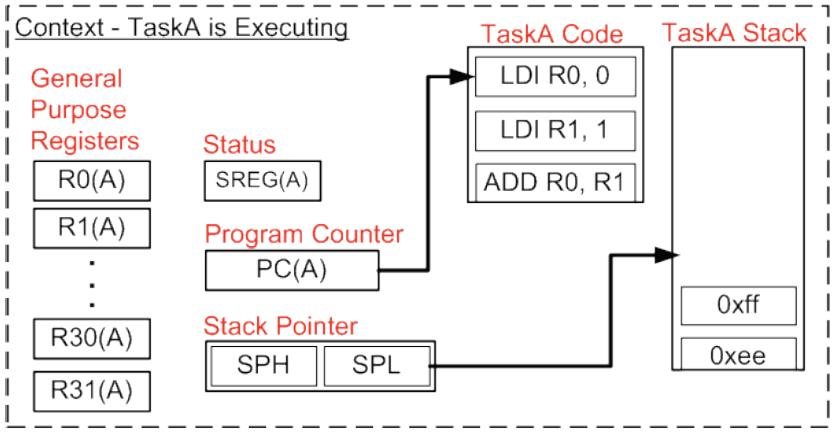
\includegraphics[width=5.5in, height=2.5in]{img/monanAVR_FigPag13_1.jpg}
$$
La etiqueta (A) en cada registro muestra que el registro contiene el valor 
correcto para la tarea A.
\subsection*{Paso 2: Ocurre la interrupción de tick del RTOS}
El tick del RTOS ocurre justo cuando TaskA está a punto de ejecutar una 
instrucción LDI. Cuando la interrupción ocurre el AVR automaticamente coloca 
el contador de programa (PC) sobre la pila antes de saltar al inicio de la ISR 
del tick del RTOS.
$$
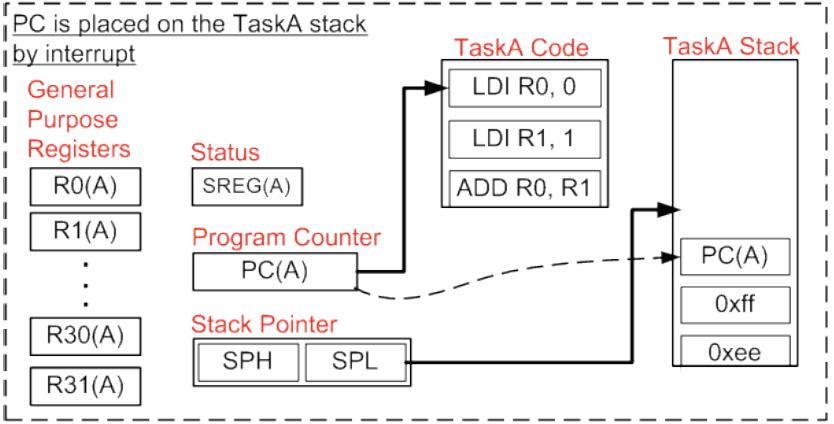
\includegraphics[width=5.5in, height=2.5in]{img/monanAVR_FigPag13_2.jpg}
$$
\subsection*{Paso 3: Se ejecuta la interrupción de tick del RTOS}
El código de aplicación ISR se muestra a continuación.
\begin{verbatim}
/* Interrupt service routine for the RTOS tick. */

void SIG_OUTPUT_COMPARE1A( void )
{
    vPortYieldFromTick();
    asm volatile ( "reti" );
}
/*-----------------------------------------------------------*/

void vPortYieldFromTick( void )
{
    portSAVE_CONTEXT();
    if( xTaskIncrementTick() != pdFALSE )
    {
        vTaskSwitchContext();
    }
    portRESTORE_CONTEXT();

    asm volatile ( "ret" );
}
/*-----------------------------------------------------------*/
\end{verbatim}
{\tt SIG$\_$OUTPUT$\_$COMPARE1A()} es una función naked, así que la primera 
instrucción es llamar a {\tt vPortYieldFromTick()}. {\tt vPortYieldFromTick()} 
es también una función naked así que el contexto de ejecución AVR es guardado 
explícitamente con una llamada a {\tt portSAVE$\_$CONTEXT()}.
\noindent
{\tt portSAVE$\_$CONTEXT()} guarda el contexto de ejecución AVR completo sobre 
la pila de TaskA, resultando en la pila ilustrada abajo. El apuntador de pila 
para TaskA ahora apunta a la cima de su propio contexto. {\tt portSAVE$\_$CONTEXT()} 
se completa almacenando una copia del apuntador de pila.El kernel ya tiene 
copia del apuntador de pila de TaskB -- tomado de la última vez que TaskB 
fue suspendida.
$$
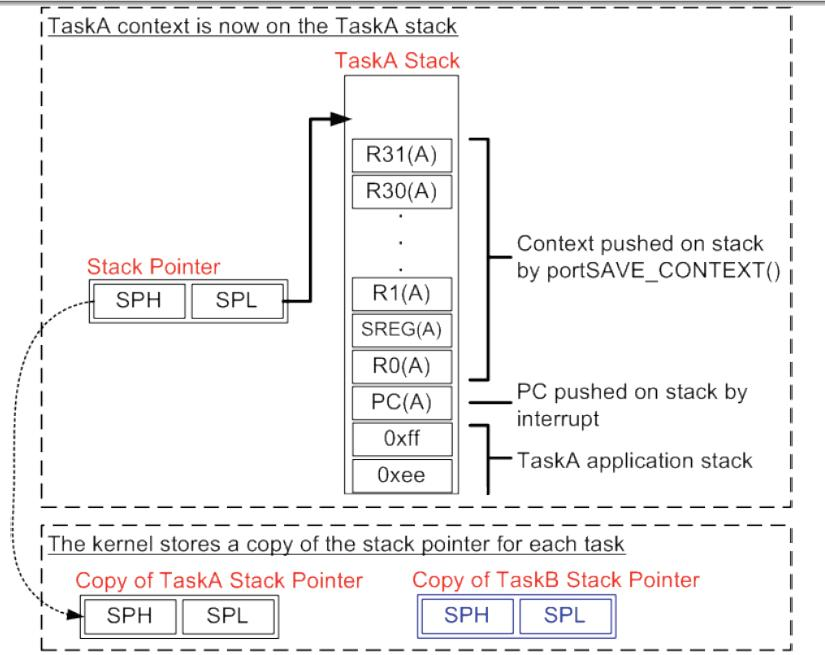
\includegraphics[width=5.5in, height=5.5in]{img/monanAVR_FigPag14.jpg}
$$
\subsection*{Paso 4: Incrementado la cuenta de Tick}
{\tt xTaskIncrementTick()} se ejecuta después de que el contexto de TaskA ha sido 
guardado. Para los propósitos de este ejemplo suponga que el incremento de la 
cuenta de tick ha causado que TaskB se ponga en estado de lista para correr. 
TaskB tiene prioridad más alta que TaskA así que {\tt vTaskSwitchContext()} 
selecciona TaskB como la tarea a la que se le debe dar tiempo de procesamiento 
cuando la ISR se complete.
\subsection*{Paso 5: Se consigue el apuntador de TaskB}
El contexto de TaskB debe ser restaurado. La primer cosa que \\
{\tt portRESTORE$\_$CONTEXT()} hace es conseguir el apuntador de pila de TaskB de
la copia tomadacuando TaskB fue suspendida. El apuntador de pila de TaskB es 
cargado en el apuntador de pila del AVR, así que ahora el apuntador de pila del AVR 
apunta a la cima del contexto de TaskB.
$$
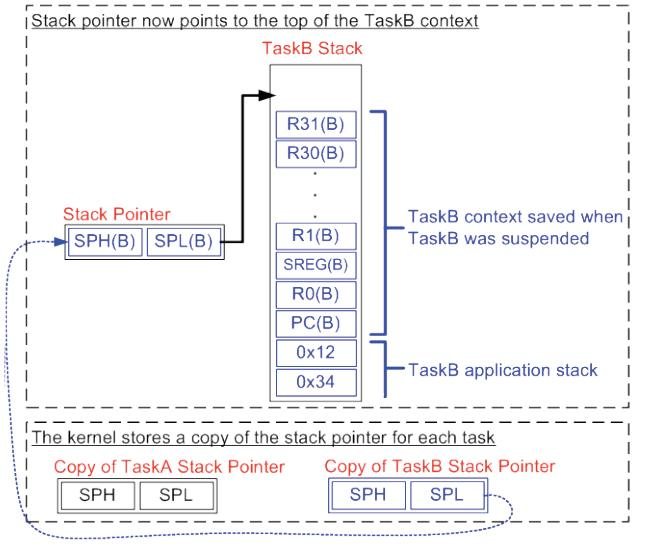
\includegraphics[width=5.5in, height=6.0in]{img/monanAVR_FigPag15.jpg}
$$
\subsection*{Paso 6: Restaurar el contexto de TaskB}
{\tt portRESTORE$\_$CONTEXT()} se completa restaurando el contexto de TaskB de 
su pila en los registos del microcontrolador adecuados.
$$
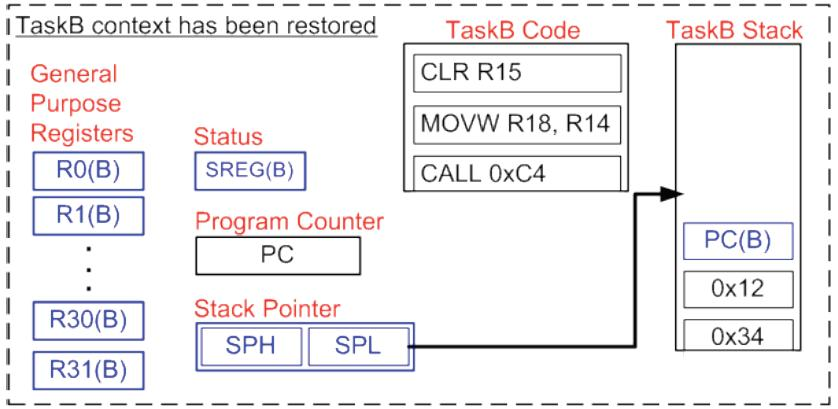
\includegraphics[width=5.5in, height=2.25in]{img/monanAVR_FigPag16_1.jpg}
$$
Solo el contador de programa permanece sobre la pila.
\subsection*{Paso 7: El RTOS tick termina}
{\tt vPortYieldFromTick()} retorna a {\tt SIG$\_$OUTPUT$\_$COMPARE1A()} donde la 
instrucción final es un retorno de interrupción (RETI). Una	instrucción RETI asume 
que el siguinete que el siguiente valor sobre la pila es una dirección de retorno 
colocada sobre la pila cuando la interrupción ocurrió.

Cuando la interrupción de tick dle RTOS empezó el AVR automaticamente colocó la 
dirección de retorno de TaskA sobre la pila -- la dirección de la siguiente 
instrucción a ejecutar en TaskA. La ISR alteró el apuntador de pila de tal manera 
que ahora apunta a la pila de TaskB. Por lo tanto la dirección de retorno extraida 
de la pila por la instrucción RETI es realmente la dirección de la instrucción de 
TaskB que se iba a ejecutar justamente antes de que fuera suspendida.
$$
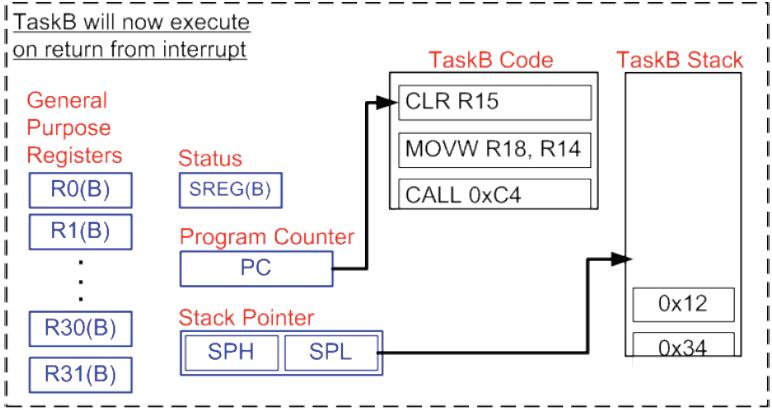
\includegraphics[width=5.5in, height=2.25in]{img/monanAVR_FigPag16_2.jpg}
$$
La interrupción de tick del RTOS interrumpió TaskA, pero está retornando a TaskB 
-- !`el cambio de contexto está compĺeto!
\AVISO
\end{document}
